\documentclass [52pt] {article}
\usepackage{amsthm}
\usepackage[margin=1in]{geometry}
\usepackage{inputenc}
\usepackage{amsmath}
\usepackage{bm}
\usepackage{afterpage}
\newcommand{\norm}[1]{\left\lVert#1\right\rVert}
\newcommand{\upn}{^{(n)}}
\newcommand{\R}{\mathbb{R}}
\newcommand{\Exp}{\mathbb{E}}
\newcommand{\basis}{\text{span}}
\newcommand{\Hil}{\mathbf{H}}
\newcommand{\trace}{\text{trace}}
\newcommand{\var}{\text{Var}}
\newcommand{\cov}{\text{Cov}}
\newcommand{\simiid}{\overset{\text{iid}}{\sim}}
\newcommand{\Prob}{\mathbb{P}}
\usepackage{ams symb}
\usepackage{enumerate}
\usepackage{amsrefs}
\usepackage{graphicx}
\usepackage{listings}
%\usepackage{atbegshi}% http://ctan.org/pkg/atbegshi
%\AtBeginDocument{\AtBeginShipoutNext{\AtBeginShipoutDiscard}}
\title{Comparing Hitting Talent Accross Different Baseball Leages}
\author{Lee Przybylski}

\begin{document}
\maketitle

\section{Comparing Leagues}
\begin{figure}[h!]
\centering
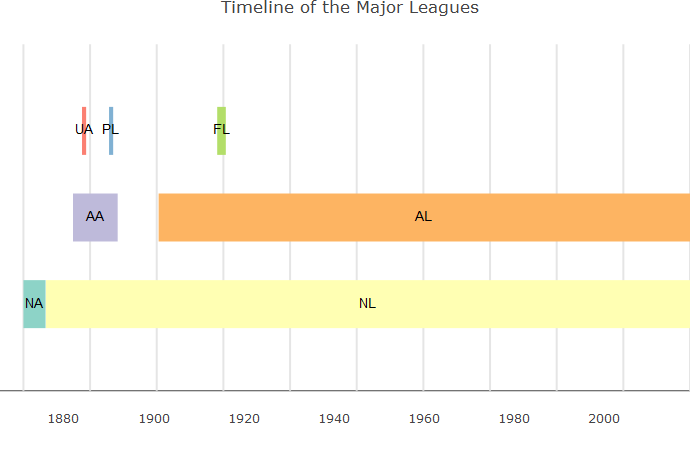
\includegraphics[scale = 0.7]{MLBtimeline.png}
\caption{\label{fig : mlbtimeline} A rough timeline for the seven leagues considered as the Major Leagues.}
\end{figure}
\noindent
We explore the prospect of comparing hitting talent accross diffent leagues using the Lahman database, available in the \verb|Lahman| package in \verb|R|.   We will first try to recreate the findings of Richard Cramer first published in the 1980 \emph{Baseball Research Journal} where he showed that average batting skill improved over the years by comparing players who played in the same league accross consecutive years.  This article can be found at
\begin{verbatim}
https://ourgame.mlblogs.com/average-batting-skill-through-major-league-history-landmarks
-of-sabermetrics-part-i-bb5849adae0b
\end{verbatim}
We will treat the American and National Leagues (AL and NL) as two different leagues and we can compare the two leagues to each other.  We can also use the same method to compare different seasons of the same league.  When we model $OPS$ for a particular player in a particular league, our model will only use data from a span of 2 years, because we want to limit ourselves to the moderate assumption that a hitter's ability does not change significantly between two consecutive seasons.  This will allow us to compare consecutive seasons directly.  Indirect comparisons will be based on different models.  
\\\\
In each model, we want to determine two test statistics, one to represent the differences in two different league effecs on $OPS$ and one to represent the differences in average hitter talent.  For the purposes of discussion, we denote our players by $i = 1,2,...,n$ and leagues by $j = 1,2,...,m$.  Each league has its own roster of players.  We denote the fact that player $i$ is played in league $j$ by $i\in L_j$.  We let $n_j$ denote the number of players in league $j$.

\section{The $OPS$ Distribution}\label{subsec : ops}
$OPS$ stands for on base plus slugging percentage.  It is defined as
\[OPS :=\frac{H+BB+HBP}{AB+BB+HBP+SF} +\frac{TB}{AB}.\]
Just as its name suggests, this is on base percentage ($OBP$)  plus slugging percentage ($SLUG$).  We refer to any plate appearance counted as an at-bat, base on balls, hit by pitch, or sacrifice fly as a batter's attempt.  Sacrifice bunts do not count as batter's attempts.  Let $n$ equal the number of attempts, so $n = AB+BB+HBP+SF$.  Given a batter playing a season in a given league, we define the following parameters: $p_w$ equals the probability that a single batter's attempt results in a walk or a hit by pitch, $p_j\:\: (j = 1,2,3,4)$ is the probability that a single batter's attempt results in a hit that advances the batter to the $j$th base,  ($p_1$ is the probability the batter hits a single etc.), and $p_B= p_1+p_2+p_3+p_4+p_w$.  We let $p_0$ denote the probabilty that a player's plate appearance results in an at bat but not a hit.  This would include strikeouts, ground outs, and reaching base by a fielding error.  Finally, we let $p_s$ denote the probability that a player's plate appearnce results in a sacrifice fly or sacrifice hit.  These instances do not count as at-bats.  We have 
\[p_s+p_w+p_0+p_1+p_2+p_3+p_4 = 1\]
so our model has six parameters, $\pmb\theta = (p_s,p_w,p_1,,p_2,p_3,p_4)'$.  These are readilly estimated using the standard statistics for a hitter in a given season.  For example, $\hat{p}_w = \frac{BB+HBP}{n}$, $\hat{p}_s = \frac{SF + SH}{n}$, etc.  According the model,
\[ \Exp[OBP] = \Exp\left[\frac{H+BB+HBP}{n}\right]= {p}_B\]
so $OBP=\hat{p}_B$ is an estimator of of $p_B$.  We also have
\[\text{Var}[OBP] = \frac{p_B(1-p_B)}{n}.\] 
We can model $TB$ as a multinomial distribution, meaning a sum of $n$ i.i.d. trials of $A_j$ such that $P[A = j] = p_j$ for $j = 0,1,2,3,4$ as defined above.  Since 
\[\Exp[A_j] = p_1+2p_2+3p_3+4p_4.\]
we get $TB= n\hat{p}_1 + 2n\hat{p}_2+3np_3+4n\hat{p}_4$ and 
\[\Exp[TB] = np_1+2np_2+3np_3+4np_4.\]
Since $AB = n(1-\hat{p}_w-\hat{p}_s)$, we find that 
\[SLUG = \frac{n(\hat{p}_1+2\hat{p}_2+3\hat{p}_3+4\hat{p}_4)}{n(1-\hat{p}_w)}=\frac{\hat{p}_1+2\hat{p}_2+3\hat{p}_3+4\hat{p}_4}{1-\hat{p}_w-\hat{p}_s}.\]
Putting everything together, 
\[OPS = \hat{p}_w+\hat{p}_1 + \hat{p}_2+\hat{p}_3+\hat{p}_4+\frac{\hat{p}_1+2\hat{p}_2+\hat{p}_3+\hat{p}_4}{1-\hat{p}_w-\hat{p}_s}.\]
Using Taylor's theorem, we can show that 
\begin{equation}\label{eq : expOPS}
\Exp[OPS] \approx  p_w+p_1 + p_2+p_3+p_4+\frac{p_1+2p_2+3p_3+p_4}{1-p_w-p_s}
\end{equation}
and
\begin{equation}\label{eq : varOPS}
\var[OPS] \approx D'\var[\hat{\pmb{\theta}}]D, 
\end{equation}
where
\[D = \begin{bmatrix}\frac{\partial OPS}{\partial p_s}\\[0.5em]
 \frac{\partial OPS}{\partial p_w}\\[0.5em]
\frac{\partial OPS}{\partial p_1}\\[0.5em]
\frac{\partial OPS}{\partial p_2}\\[0.5em] \frac{\partial OPS}{\partial p_3}\\[0.5em]
\frac{\partial OPS}{\partial p_4}\\\end{bmatrix}
=\begin{bmatrix}
\frac{p_1+2p_2+3p_3+4p_4}{(1-p_w-p_s)^2}\\[0.5em]
1+\frac{p_1+2p_2+3p_3+4p_4}{(1-p_w-p_s)^2}\\[0.5em]
1+\frac{1}{1-p_w-p_s}\\[0.5em]
1+\frac{2}{1-p_w-p_s}\\[0.5em]
1+\frac{3}{1-p_w-p_s}\\[0.5em]
1+\frac{4}{1-p_w-p_s}\\
\end{bmatrix}.\]
To understand $\var[\hat{\pmb{\theta}}]$, first observe that for one of our parameters $p_i$, 
\[\Exp[\hat{p}_i] =p_i,\:\:\:\var[\hat{p}_i]=\frac{p_i(1-p_i)}{n}.\]  
For two different parameters, $p_i$ and $p_k$, we find their covariance by first defining $B_{ij}$ as 1 if the event corresponding to $i$ occurred at the $j$th at bat, and 0 otherwise.  We define $B_{kj}$ in basically the same way.  Thus
\[\hat{p}_{i} = \frac{1}{n}\sum_{j=1}^n B_{ij},\:\:\hat{p}_{k} = \frac{1}{n}\sum_{j=1}^n B_{kj}.\]
Thus,
\[\begin{split}
\cov[\hat{p}_i,\hat{p}_k] &= \Exp[\hat{p}_i\hat{p}_k]-\Exp[\hat{p}_i]\Exp[\hat{p}_k] = \frac{1}{n^2}\sum_{j=1}^n\sum_{l=1}^n\Exp[B_{ij}B_{kl}] - p_ip_k=\frac{1}{n^2}\sum_{1\le l\not= j\le n} \Exp[B_{ij}]\Exp[B_{kl}]-p_ip_k\\
&=\frac{1}{n^2}\sum_{1\le l\not= j\le n} p_ip_k -p_ip_k=\frac{n^2-n}{n^2} p_ip_k -p_ip_k = -\frac{1}{n}p_i p_k
\end{split}.\]
We note that the third equality above is due to the fact that the events used to define $p_i$ and $p_k$ cannot happen simultaneously, and events corresponding to different plate appearances are assumed to be independent.  Hence 
\[\var[\hat{\pmb{\theta}}] =n^{-1}\begin{bmatrix}
p_s(1-p_s) & -p_sp_w& -p_sp_1 & -p_sp_2 & -p_s p_3& -p_s p_4\\[0.5em]
& p_w(1-p_w)& -p_wp_1 & -p_wp_2& -p_wp_3 & -p_w p_4\\[0.5em]
&& p_1(1-p_1)& -p_1p_2& -p_1p_3& -p_1p_4\\[0.5em]
&&& p_2(1-p_2) & -p_2p_3& -p_2p_4\\[0.5em]
&&&& p_3(1-p_3) & -p_3p_4\\[0.5em]
&&&&&p_4(1-p_4)\\
\end{bmatrix}\]
From (\ref{eq : varOPS}), this suggests that $\var[OPS] =\frac{\sigma^2}{n}$ for some $\sigma^2>0$. \\

\section{Linear Model Selection}
In this section, we consider a series of linear models to estimate the true mean of $OPS$ for a given player in a given league.  Our models assume there is a portion of the mean that is attributed to the player and another portion of the mean that results from the players environment.  Estimates of the term that is unique for the player give us an estimate of the player's talent.  Due to the theoretical result in the previous section, we suspect that the variance is inversely related to the number of plate appearances.  We find in practice that this is not exactly the case.  To illustrate this, we fit an unweighted model to the Lahman data from 1899 to 1972.  This model is given by
\begin{equation}\label{eq : unwtd_model}
OPS_{ijk} = \mu+\rho_i+\lambda_{jk} +\varepsilon_{ijk}, \:\:\varepsilon_{ijk}\sim N(0, \sigma^2).
\end{equation}
where $OPS_{ij}$ $OPS$ for player $i$ playing in league $j$ during season $k$.  In our code, we avoid singularities by creating a new factor, \verb|lg.yr| by pasting the name of the league to the season for each observation.  This makes sense since not every league plays in every season.  We then obtain the residuals of model (\ref{eq : unwtd_model}).  We expect that a weighted model will have standard deviation proportional to a power of the number of plate appearances, that is, 
\[\var[OPS_{ijk}] = PA_{ijk}^{\theta}\sigma^2\]
for some $\theta <0$.  Equivalently, 
\[\log(\text{Var}[OPS_{ijk}]) = {\theta}\log(PA_{ijk}) + 2\log(\sigma).\]
Thus we can estimate $\theta$ by performing a linear regression of the log of the squared residuals of the unweighted model with respect to $\log(PA)$.  When doing this, we notice that a collection of the squared residuals are extremely small.  These are for the instances where we only observe a player once.  With one observation, it is impossible to get a reasonable estimate of the player's effect on $OPS$.  This will also be common in the college baseball data.
\\\\
A major problem with (\ref{eq : unwtd_model}) is that for players that have only one observation, the residual is very small.  This is because there many observations of a particular league-year, but only one observation for the player.

Because of how common it is for us to have few observations of a single player, we would like to consider a model with random player effects.  Consider
\begin{equation}\label{eq : rand_player_model}
OPS_{ijk} = \mu+\lambda_{jk} + p_i+\varepsilon_{ijk}PA_{ijk}^{-1/2}, \:\:p_i\sim N(0,\sigma^2_p),\:\varepsilon_{ijk}\sim N(0, \sigma^2).
\end{equation}

\subsection{Linear Player Age}
Our first model considers

\section{A Player and League Effects Model}\label{sec : att2}

Looking at the theoretical result in the previous section provides some insight about the variance for a linear model predicting $OPS$.  The amount of variance for $OPS$ under a given observation should be inversely related to the number of plate appearances.  Thus we consider the model
\begin{equation}\label{eq : model2}
OPS_{ij} = \mu+\rho_i+\lambda_{jk} +\varepsilon_{ijk}PA_{ij}^{-1/2}, \:\:\varepsilon_{ijk}\sim N(0, \sigma^2).
\end{equation}
Here, $\lambda_{jk}$ is the league effect on $OPS$ for league $j$ in year $k$.  The $\rho_i$ denotes the effect of player $i$ on $OPS$. One concern is that the player effect might also change over time, but for now we ignore this.  

The additive model in (\ref{eq : model2}) give us a natural way to quantify the the differences in league effects on $OPS$ and the differences in average hitting ability between players of different leagues.  First, suppose we would like to know if the the league effect on $OPS$ in the $j$th league has a significant change after the $k$th season.  The null hypothesis associated with this question is 
\[H_0: \lambda_{jk} = \lambda_{j(k+1)}\]
We test this with a t-statistic.  We could also compare how easy or difficult it is for hitters in different leagues accross the same season.  The null hypothesis related to this question is 
\[H_0: \lambda_{j_1k} = \lambda_{j_2k} = ...= \lambda_{j_nk}.\]
This can be tested using an F-statistic.  To do this we construct a matrix $C$, with $n - 1$ rows such that 
\[C\hat{\pmb{\beta}} = (\lambda_{j_1k}-\lambda_{j_2k},\lambda_{j_1k}-\lambda_{j_3k}, ..., \lambda_{j_1k}-\lambda_{j_nk})'\] 
where $\hat{\pmb{\beta}}$ is the vector of parameter estimated from the model.  The hypothesis is equivalent to 
\[H_0:C\pmb\beta = \mathbf{0}.\]

To address questions about how talented the hitters are in a given league, we define the average hitting talent in league $j$ during season $k$ as
\[\Theta_{jk} = \frac{1}{n}\sum_{i\in L_{jk}} p_i.\]
This is just an average of the player effects for those players belonging to league $j$ in the $k$th season.  If we want to know if hitting talent in league $j$ has changed between two consecutive seasons, we can test the null hypothesis
\[H_0: \Theta_{jk} = \Theta_{j,k+1}\]
using a t-statistic.  The final question we might ask is if the average hitting talent was different between the different Major Leagues in a given season.  The null hypothesis associated with this question is 
\[H_0: \Theta_{j_1k} = \Theta_{j_2k} = ...= \Theta_{j_nk}.\]
Just as we did with league effects, this is easily tested with an F-statistic. 

 In the plot of hitting talent, during the seasons where there is a significant difference in average hitting talent among the leagues in a given season, the seasons are plotted with a ``$*$".

If the null hypothesis is rejected, we connect the seasons with a solid line instead of a dashed line in the plot.  This means the change in how difficult it was to hit in the league was significant between these two seasons.    As with the question about league effects, we connect the seasons on the plot with a solid line instead of a dashed line.  In the plot of league effects on $OPS$, during the seasons where there is a significant difference between the different leagues in a season, those seasons are plotted with a ``$*$".  


We can perform season to season comparisons by fitting model (\ref{eq : model2}) to two seasons of data at a time.  By repeating this for all seasons from 1871 to 2018, we can compare consecutive seasons.Below we plot the year to year league effects and comparisons of average hitting ability for the Major Leagues under this model.  In the league effects plot, we add vertical lines for the following years that had significant rule changes that we might expect to  have effected $OPS$ uniformly for all players in a league:
\begin{itemize}
\item1884 - Pitchers were allowed to deliver the ball overhand.
\item 1889- The modern rule of 4 balls or 3 strikes is first used.  In 1887 for example, players were allowed 4 strikes.
\item 1893 - The pitcher is moved back from a pitchers box that is 50 ft from home plate to a rubber that is 60 ft 6 in from home.
\item 1901 - Foul balls begin to count as strikes.  This is first implemented in the NL and in 1903 it is also implemented in the AL.
\item1969 - After an offensively frustrating season where Carl Yastrzemski lead the AL with a .301 $BA$, the mound was lowered from 15 to 10 inches high and the top of the strike zone is lowered from the top of the hitter's shoulders to his armpits.
\end{itemize}
\begin{figure}[h!]
\centering
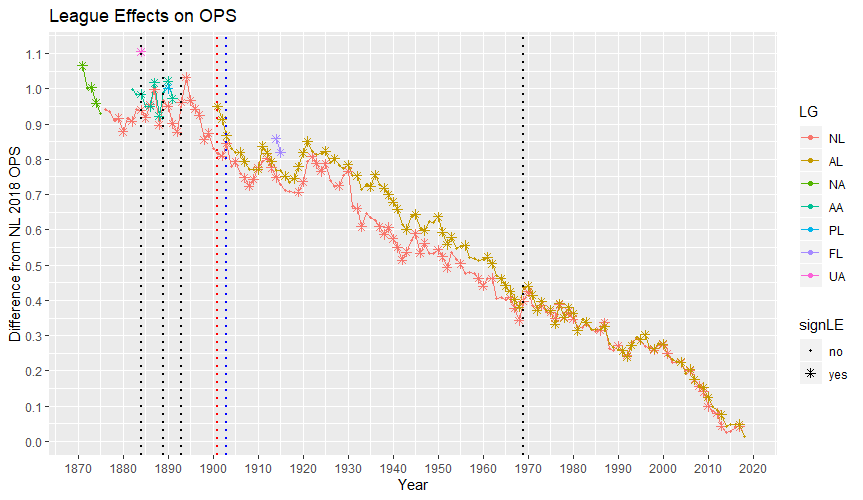
\includegraphics[scale = 0.75]{MLByr2yrLE_v2.png}
\caption{\label{fig : LEv2} Year to year comparisons of league effects on $OPS$ for the seven historical major leagues using model (\ref{eq : model2}).  }
\end{figure}
\begin{figure}[h!]
\centering
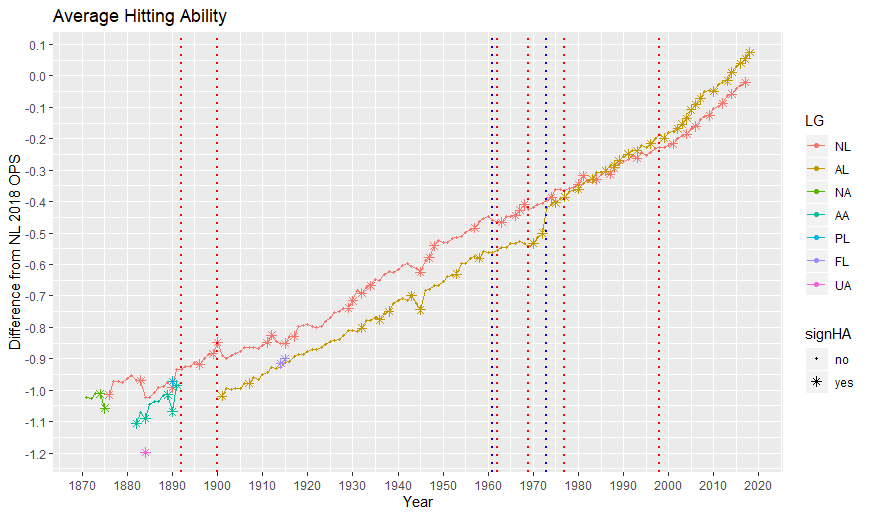
\includegraphics[scale = 0.7]{MLByr2yrHA_v2.png}
\caption{\label{fig : HAv2} Year to year comparisons of average hitting ability based on $OPS$ for the seven historical major leagues using model (\ref{eq : model2}).  Red vertical lines indicate a change in the number of NL teams.  Blue vertical lines indicate a change in the number of AL teams.}
\end{figure}
To better understand how to interpret these statistics, look at the following output:
\begin{verbatim}
> d.comps[d.comps$start.yr == 1972,c(3:5,7:8,10:11)]
         LG1     LG2        LG.ef     LE.pval     Tal.diff      TD.pval comn.plyrs
1081 NL.1972 NL.1973 -0.009365313 0.214909632 -0.010504143 1.382065e-01        218
1082 NL.1972 AL.1973 -0.017349391 0.345697916 -0.072911588 5.635844e-05         30
1083 NL.1972 AL.1972  0.006797458 0.719799481  0.007182892 7.049179e-01          9
1084 NL.1973 NL.1972  0.009365313 0.214909632  0.010504143 1.382065e-01        218
1085 NL.1973 AL.1973 -0.007984077 0.672203915 -0.062407445 7.069133e-04         12
1086 NL.1973 AL.1972  0.016162772 0.402741540  0.017687035 3.564599e-01         20
1087 AL.1973 NL.1972  0.017349391 0.345697916  0.072911588 5.635844e-05         30
1088 AL.1973 NL.1973  0.007984077 0.672203915  0.062407445 7.069133e-04         12
1089 AL.1973 AL.1972  0.024146849 0.002500686  0.080094480 0.000000e+00        165
1090 AL.1972 NL.1972 -0.006797458 0.719799481 -0.007182892 7.049179e-01          9
1091 AL.1972 NL.1973 -0.016162772 0.402741540 -0.017687035 3.564599e-01         20
1092 AL.1972 AL.1973 -0.024146849 0.002500686 -0.080094480 0.000000e+00        165
\end{verbatim}
The columns \verb|LG1| and \verb|LG2| indicate the two leagues being compared.  The column \verb|LG.ef| indicates the estimated difference in the league effects on $OPS$ and \verb|LE.pval| indicates the p-value associated with this estimate.  The column \verb|Tal.dff| indicates the estimated difference in the average hitter's effect on $OPS$ and \verb|TD.pval| is the associated p-value.  The first row tells us that the 1972 NL was more difficult to hit in league wide by about 0.009 $OPS$ although this difference is not statistically significant.  Similarly the average hitter's effect was smaller by 0.011 $OPS$ and this difference was not statistically significant.  If anything changed in the NL between these two years, the evidence says that the averge hitter got slightly better in 1973.  The last row of the output suggests that things also got easier for hitters in the AL between 1972 and 1973 by about 0.024 $OPS$ which was a significant difference.  On the other hand, the ability of the average hitter is estimated to have significantly improved by 0.080, which is probably due to the designated hitter rule.
\\\\
Comparing these results to the results in Cramer's study, we might be a bit uneasy.  The steps that we obtain using our model are larger.  There are some key differences that add some confusion.  Cramer bases his comparisons on batter win average, which is not defined in his article, and when he makes a season to season comparison, he only uses players who play in both leagues.  In order to better compare our method with Cramer's we perform the same comparisons as in model (\ref{eq : model2}) but with $BA$ as the output instead.  I have also changed the column \verb|rel.HA| to represent the average hitting talent in the league compared to the NL in 1976, just as in the table provided by Cramer.  Notice our difference in batting average for the NL in 1960 is -0.0396 where Cramer estimated it to be -0.004, and for the AL it was -0.0943 where Cramer's estimate was -0.017.  If we go all the way back to the first NL season, 1876, we get a difference of -0.2951, where Cramer came up with -0.123.  Our number suggests that the average player from the first season of the NL would almost never get a hit in the 1976 season.  This might be possible considering the 1876 rules still required the pitcher to deliver the ball underhanded and players did not wear gloves in the field, but it still seems like a stretch.
\begin{verbatim}
 LG   YR       rel.HA     HA.pval LG   YR       rel.HA      HA.pval
 NL 1979  0.007498388 0.214128013 AL 1979 -0.001443420 3.805310e-01
 NL 1978  0.005015233 0.281706810 AL 1978 -0.003056244 4.201078e-01
 NL 1977  0.002595796 0.397728412 AL 1977 -0.010337636 1.522183e-03
 NL 1976  0.000000000 0.327069418 AL 1976 -0.015861695 2.211858e-02
 NL 1975 -0.001332416 0.582842733 AL 1975 -0.020554222 7.395716e-02
 NL 1974 -0.009789343 0.002410404 AL 1974 -0.024711244 6.975659e-02
 NL 1973 -0.013974676 0.146479945 AL 1973 -0.030179950 3.652036e-02
 NL 1972 -0.020028541 0.018183812 AL 1972 -0.056184474 1.110223e-15
 NL 1971 -0.024206956 0.094175827 AL 1971 -0.064344813 3.612706e-03
 NL 1970 -0.026907561 0.306337503 AL 1970 -0.071208198 1.490615e-02
 NL 1969 -0.029372613 0.381022898 AL 1969 -0.077498498 1.931780e-02
 NL 1968 -0.023853880 0.028040788 AL 1968 -0.076551146 7.146779e-01
 NL 1967 -0.032935080 0.003328016 AL 1967 -0.074191418 4.035065e-01
 NL 1966 -0.038655497 0.048057140 AL 1966 -0.078228096 1.072795e-01
 NL 1965 -0.038101694 0.849250471 AL 1965 -0.080221265 5.160448e-01
 NL 1964 -0.037562652 0.849086529 AL 1964 -0.085551282 8.699337e-02
 NL 1963 -0.044375507 0.025692892 AL 1963 -0.087909936 4.275607e-01
 NL 1962 -0.043614973 0.782429847 AL 1962 -0.090259058 3.891868e-01
 NL 1961 -0.041620493 0.530123887 AL 1961 -0.091816095 6.255709e-01
 NL 1960 -0.039595488 0.543317632 AL 1960 -0.094259275 4.390831e-01
\end{verbatim}
It might be that there are not enough observations in two seasons to accurately assess the effect of each hitter.  We relax the assumptions that player effects change every season and fit the model using every season in the Lahman data.  Each player is assigned a parameter $\rho_i$.  The league effects $\lambda_j$ are indexed by both the league and the year.  This is done by creating a new factor, \verb|lg.yr|, by pasting the name of the league and the year for each observation. This fit took just under 50 minutes.  The results seem a little more reasonable since the range of league effects and player effects is smaller, close to 0.6.  In figure \ref{fig : plyrlg_LE2} we plot the league effects relative to the 1976 season of the NL, and in figure \ref{fig : plyrlg_HA2} we plot the estimated hitting ability relative to the 1976 season of the NL.  It is noteworthy that according to this new fit, the AL had more hitting talent than the NL even in its first decade.  The jump in 1973 due to the DH rule is also more distinct, but it is really about the same size as in the previous fit.
\\\\
\begin{figure}[h!]
\centering
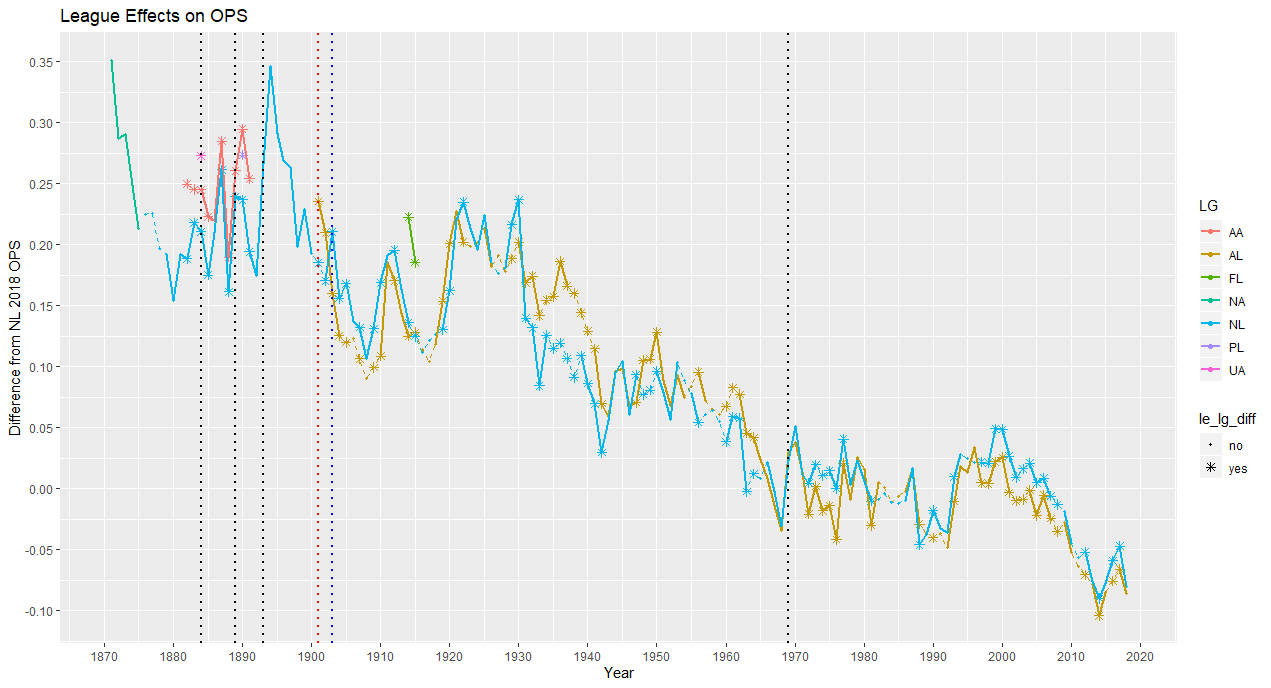
\includegraphics[scale = 0.5]{PlyrEffReg_MLB_LEplot.png}
\caption{\label{fig : plyrlg_LE2} Year to year comparisons of league effects on $OPS$ for the seven historical major leagues using model (\ref{eq : model2}) fit with all seasons of Lahman data at once.  }
\end{figure}
\begin{figure}[h!]
\centering
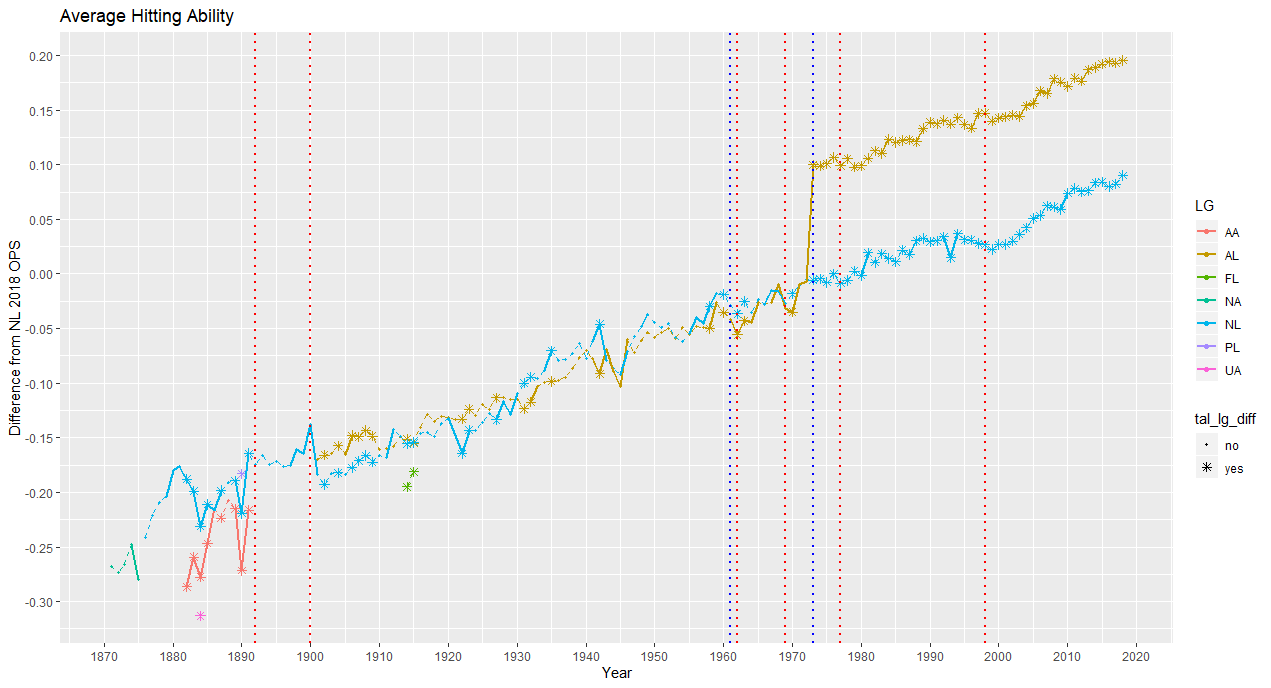
\includegraphics[scale = 0.5]{PlyrEffReg_MLB_HAplot.png}
\caption{\label{fig : plyrlg_HA2} Year to year comparisons of average hitting ability based on $OPS$ for the seven historical major leagues using model (\ref{eq : model2}).  This fit uses all seasons of Lahman data at once.}
\end{figure}
\noindent An interesting observation from figure \ref{fig : plyrlg_HA2} is that it is more common for the difference between leagues to be significant during a given season than for the average talent to change significantly between two seasons.  Perhaps this makes sense since great hitters typically have longer careers than great pitchers.  Great pitchers are not always great for their entire career either.  They might get hurt or the league just figures out how to handle them.  Pitching ability is probably a significant factor in determining the league effects on OPS, so this quantity should be less stable season after season.  You can see how the DH rule produced a significant change in average hitting talent for the AL.  According to the model, if we estimate the average hitting talent in AL 1973 minus the average hitting talent in AL 1972 we get a 95\% confidence interval of (0.0953, 0.1189).

\end{document}